% Project GAIA — Threat Model & Defense Pipeline (TikZ)
% IEEEtran conference double-column figure
\begin{figure*}[t]
\centering
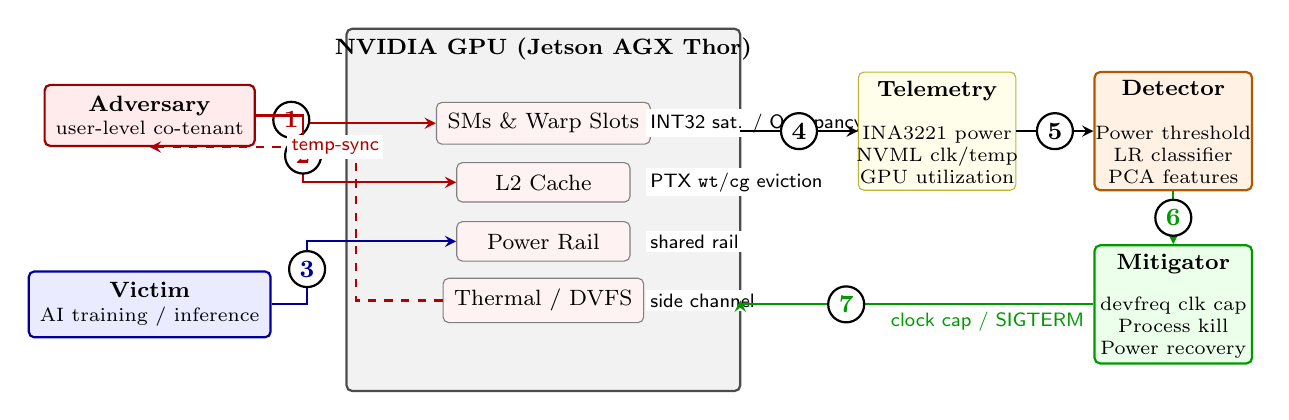
\begin{tikzpicture}[
    >=stealth,
    every node/.style={font=\footnotesize},
    box/.style={draw, rounded corners=2pt, minimum height=0.65cm,
                align=center, fill=#1, inner sep=4pt},
    box/.default=white,
    attackbox/.style={box=red!8, draw=red!60!black, thick},
    victimbox/.style={box=blue!8, draw=blue!60!black, thick},
    gpubox/.style={box=gray!10, draw=black!70, thick},
    detectbox/.style={box=orange!10, draw=orange!70!black, thick},
    mitigatebox/.style={box=green!8, draw=green!60!black, thick},
    telbox/.style={box=yellow!8, draw=yellow!70!black},
    resbox/.style={box=red!5, draw=gray, minimum width=2.2cm, minimum height=0.5cm},
    lbl/.style={font=\scriptsize\sffamily, fill=white, inner sep=1.5pt},
    cnum/.style={circle, draw=black, fill=white, font=\scriptsize\bfseries,
                 inner sep=0.5pt, minimum size=13pt},
    arr/.style={->, thick},
    darr/.style={->, thick, dashed},
]

% ===== LEFT: ACTORS =====
\node[attackbox, minimum width=2.2cm] at (0, 1.2)
    (attacker) {\textbf{Adversary}\\[-1pt]{\scriptsize user-level co-tenant}};

\node[victimbox, minimum width=2.2cm] at (0, -1.2)
    (victim) {\textbf{Victim}\\[-1pt]{\scriptsize AI training / inference}};

% ===== CENTER: GPU =====
\node[gpubox, minimum width=5.0cm, minimum height=4.6cm] at (5.0, 0)
    (gpu) {};
\node[font=\footnotesize\bfseries, anchor=north] at (gpu.north)
    {NVIDIA GPU (Jetson AGX Thor)};

% GPU internal resources — stacked
\node[resbox] at (5.0, 1.1) (sms)   {SMs \& Warp Slots};
\node[resbox] at (5.0, 0.35) (l2)   {L2 Cache};
\node[resbox] at (5.0,-0.4) (pwr)  {Power Rail};
\node[resbox] at (5.0,-1.15) (therm) {Thermal / DVFS};

% Resource annotations (right side of GPU sub-boxes)
\node[lbl, anchor=west] at (6.3, 1.1)
    {\scriptsize INT32 sat. / Occupancy};
\node[lbl, anchor=west] at (6.3, 0.35)
    {\scriptsize PTX \texttt{wt}/\texttt{cg} eviction};
\node[lbl, anchor=west] at (6.3,-0.4)
    {\scriptsize shared rail};
\node[lbl, anchor=west] at (6.3,-1.15)
    {\scriptsize side channel};

% ===== ATTACK VECTORS =====
% Attacker -> SMs
\draw[arr, red!70!black]
    (attacker.east) -- ++(0.45,0) |- (sms.west)
    node[cnum, pos=0.28] {\small 1};
% Attacker -> L2
\draw[arr, red!70!black]
    (attacker.east) -- ++(0.6,0) |- (l2.west)
    node[cnum, pos=0.3] {\small 2};

% Victim -> Power Rail
\draw[arr, blue!60!black]
    (victim.east) -- ++(0.45,0) |- (pwr.west)
    node[cnum, pos=0.28] {\small 3};

% Temp-sync feedback (dashed): Thermal -> Attacker
\draw[darr, red!70!black]
    (therm.west) -- ++(-1.1,0) |- (attacker.south)
    node[lbl, pos=0.55] {\scriptsize temp-sync};

% ===== TELEMETRY =====
\node[telbox, minimum width=2.0cm, minimum height=1.5cm] at (10.0, 1.0)
    (telemetry) {};
\node[font=\footnotesize\bfseries, anchor=north] at (telemetry.north)
    {Telemetry};
\node[font=\scriptsize, align=center] at (10.0, 0.7)
    {INA3221 power\\NVML clk/temp\\GPU utilization};

% GPU -> Telemetry
\draw[arr] (7.5, 1.0) -- (telemetry.west)
    node[cnum, midway] {\small 4};

% ===== DETECTOR =====
\node[detectbox, minimum width=2.0cm, minimum height=1.5cm] at (13.0, 1.0)
    (detector) {};
\node[font=\footnotesize\bfseries, anchor=north] at (detector.north)
    {Detector};
\node[font=\scriptsize, align=center] at (13.0, 0.7)
    {Power threshold\\LR classifier\\PCA features};

% Telemetry -> Detector
\draw[arr] (telemetry.east) -- (detector.west)
    node[cnum, midway] {\small 5};

% ===== MITIGATOR =====
\node[mitigatebox, minimum width=2.0cm, minimum height=1.5cm] at (13.0, -1.2)
    (mitigator) {};
\node[font=\footnotesize\bfseries, anchor=north] at (mitigator.north)
    {Mitigator};
\node[font=\scriptsize, align=center] at (13.0, -1.5)
    {devfreq clk cap\\Process kill\\Power recovery};

% Detector -> Mitigator
\draw[arr, green!60!black] (detector.south) -- (mitigator.north)
    node[cnum, midway] {\small 6};

% Mitigator -> GPU (feedback loop)
\draw[arr, green!60!black, thick]
    (mitigator.west) -| (7.5, -1.15)
    node[cnum, pos=0.35] {\small 7}
    node[lbl, pos=0.15, below=1pt] {\scriptsize clock cap / SIGTERM};

\end{tikzpicture}

\vspace{-2pt}
\caption{GAIA threat model and closed-loop defense pipeline.
A co-tenant adversary \protect\ding{192}\,saturates GPU compute units
(INT32, occupancy) and \protect\ding{193}\,thrashes the L2 cache via
PTX cache-control hints, elevating power on the \protect\ding{194}\,shared
rail where victims run.
Hardware telemetry \protect\ding{195}\,(INA3221 current sensor, NVML)
feeds a power-level detector and logistic-regression
classifier~\protect\ding{196}.
On anomaly detection, the closed-loop mitigator~\protect\ding{197}\,applies
a devfreq clock cap or terminates the adversarial process, restoring
baseline power~\protect\ding{198}.
Dashed arrow: thermal side-channel used for attack synchronization.}
\label{fig:threat}
\end{figure*}
